\documentclass[11pt]{article}
\usepackage{../common/dastyle}
\graphicspath{{../figures/}}

\title{\vspace{-1.5cm}\textbf{Adaptation de Domaine}\\[0.1cm]\Large Séance 6 --- Fouille de Données Massives}
\author{Guillaume Metzler\\[0.1cm]\small Institut de Communication (ICOM), Université Lumière Lyon 2\\ \small Laboratoire ERIC UR 3083\\[0.1cm]\small\texttt{guillaume.metzler@univ-lyon2.fr}}
\date{M2 Informatique -- SISE}

\begin{document}
\maketitle
\thispagestyle{plain}

\begin{abstract}
\noindent Que se passe-t-il quand le modèle qu'on a entraîné doit fonctionner sur des données qui ne
ressemblent plus tout à fait à celles de l'entraînement ? C'est la question de l'\emph{adaptation de
domaine} : on dispose de données \emph{source} annotées, mais on veut être performant sur un domaine
\emph{cible} différent, pour lequel on n'a pas (ou peu) d'étiquettes. Ce document introduit le cadre
formel de l'adaptation de domaine non supervisée, détaille en profondeur les méthodes de repondération
d'instances (estimation de densité, KLIEP, KMM, classifieur de domaine), puis présente les bornes de
généralisation qui expliquent \emph{pourquoi} et \emph{sous quelles conditions} ces méthodes fonctionnent
(divergence $\Hcal\Delta\Hcal$, bornes PAC-Bayésiennes), avant d'ouvrir sur les approches profondes et
récentes du domaine (DANN, transport optimal, test-time adaptation, modèles de fondation). Les bases sont
volontairement traitées avec le même niveau de détail que le notebook \texttt{Code\_DA.ipynb} du cours,
pour que les notions les plus techniques restent solidement ancrées avant d'aborder les développements
récents.
\end{abstract}

\tableofcontents

%=====================================================================
\section{Introduction : pourquoi adapter un modèle ?}
%=====================================================================

Ce premier chapitre pose le décor. Nous allons voir, sur trois exemples concrets, pourquoi un modèle
entraîné dans de bonnes conditions peut se révéler décevant une fois déployé ailleurs ; nous donnerons
ensuite un nom précis à ce qui change d'un contexte à l'autre --- le \emph{domaine} et la \emph{tâche}
--- avant de situer l'adaptation de domaine dans la famille plus large du \emph{transfer learning}, et
de préciser les hypothèses sous lesquelles on peut raisonnablement espérer transférer une connaissance
d'un domaine à un autre.

\subsection{Trois exemples qui posent le problème}

Le premier exemple vient de la reconnaissance d'objets : un système de vision entraîné avec les images
d'une caméra particulière (éclairage, angle, résolution donnés) doit, une fois déployé, fonctionner avec
une caméra différente, installée ailleurs. Les images \enquote{se ressemblent} conceptuellement --- ce
sont toujours des photographies des mêmes types d'objets --- mais leurs statistiques (couleurs,
contraste, cadrage) diffèrent sensiblement. Le deuxième exemple est linguistique : un classifieur entraîné
sur des avis clients concernant des livres doit être réutilisé pour juger des avis sur de
l'électroménager. Le vocabulaire change du tout au tout (\enquote{passionnant}, \enquote{bien écrit}
d'un côté, \enquote{silencieux}, \enquote{durable} de l'autre), mais la tâche --- détecter un avis
positif ou négatif --- reste rigoureusement la même. Le troisième exemple, enfin, est industriel : un
modèle de détection de défauts est entraîné sur des données \emph{simulées}, moins coûteuses à produire
en grand nombre, puis doit fonctionner sur des mesures réelles, dont la distribution ne coïncide jamais
tout à fait avec celle de la simulation.

Ces trois situations, bien que très différentes en apparence, partagent la même structure : on dispose
d'un domaine \emph{source} où l'apprentissage est facile --- les données y sont abondantes et
étiquetées --- et l'on souhaite être performant sur un domaine \emph{cible}, différent, où les
étiquettes sont rares, coûteuses à obtenir, voire totalement absentes. On retrouve ce schéma dans un
nombre considérable de champs applicatifs : la détection d'anomalies, la biologie, la médecine, les jeux
vidéo, la localisation intérieure ou encore le traitement du signal. Le \emph{transfer learning} n'est
donc pas une méthode isolée, mais bien une famille de problèmes qui traverse presque tout le machine
learning appliqué.

\subsection{Domaine, tâche, risque}

Pour aller plus loin, il nous faut un langage précis. Nous reprenons pour cela le formalisme standard de
l'apprentissage statistique, que nous étendons au cadre du transfert.

\begin{definition}{Domaine et tâche}{domaine}
Soit $\X$ un espace de features et $\Y$ un espace d'étiquettes, et $(X,Y)$ un couple de variables
aléatoires sur $\X\times\Y$ de loi $P$. On appelle \textbf{domaine} le couple $\D = \{\X, P(X)\}$ ---
l'espace des features et sa distribution marginale --- et \textbf{tâche} le couple $\Tcal = \{\Y,
P(Y\mid X)\}$ --- l'espace des étiquettes et la loi conditionnelle que l'on cherche à prédire.
\end{definition}

Autrement dit, le domaine décrit \enquote{à quoi ressemblent les données d'entrée} à travers la
distribution marginale $P(X)$, tandis que la tâche décrit \enquote{ce que l'on cherche à prédire} à
travers la loi conditionnelle $P(Y\mid X)$. Un même jeu de données peut ainsi changer de domaine --- les
images changent de style --- sans changer de tâche, puisqu'on cherche toujours à reconnaître un chat ;
et réciproquement.

\begin{definition}{Transfer learning}{transfer}
On appelle \textbf{transfer learning} le cadre d'apprentissage qui exploite la connaissance acquise sur
un domaine/tâche \emph{source} $(\D_S,\Tcal_S)$ pour améliorer l'apprentissage sur un domaine/tâche
\emph{cible} différent mais lié $(\D_T,\Tcal_T)$. On parle de \emph{décalage de domaine} (\textit{domain
shift}) si $\X_S \neq \X_T$ ou $P_S(X)\neq P_T(X)$, et de \emph{décalage de tâche} (\textit{task shift})
si $\Y_S\neq \Y_T$ ou $P_S(Y\mid X)\neq P_T(Y\mid X)$.
\end{definition}

Pour comparer des modèles entre eux, il nous faut aussi rappeler la notion de risque, familière depuis
le début du cours.

\begin{definition}{Risque d'un classifieur/régresseur}{risque}
Pour une fonction de perte $\ell:\Y\times\Y\to\R$ et une hypothèse $h:\X\to\Y$, le risque de $h$ sous une
distribution $P$ est
\[
R(h) = \Esp{(X,Y)\sim P}{\ell(h(X),Y)}.
\]
En pratique, on ne connaît $P$ qu'à travers un échantillon i.i.d. $\{(x_i,y_i)\}_{i=1}^N$, et on minimise
le risque empirique $\widehat R(h) = \frac1N\sum_{i=1}^N \ell(h(x_i),y_i)$ (principe ERM).
\end{definition}

Muni de ces définitions, le point de départ de tout ce cours tient en une phrase, aussi simple que
fondamentale : dès que $P_S \neq P_T$, le risque source $R_S(h)$ et le risque cible $R_T(h)$ sont deux
quantités \emph{différentes}. Minimiser $\widehat R_S(h)$, ce que l'on sait très bien faire, n'a donc
\emph{aucune raison a priori} de minimiser $R_T(h)$, ce que l'on veut vraiment faire. Tout l'enjeu de
l'adaptation de domaine consiste précisément à relier ces deux risques l'un à l'autre.

\subsection{Pourquoi ne pas simplement réentraîner sur la cible ?}

On pourrait légitimement se demander pourquoi ne pas tout simplement oublier la source et entraîner un
modèle directement sur la cible. En pratique, cette stratégie échoue le plus souvent, et ce pour
plusieurs raisons qui se combinent souvent entre elles. D'abord, on dispose fréquemment de très peu de
données cible : l'annotation peut être coûteuse, lente, voire dangereuse --- pensons à la détection de
pannes rares sur une infrastructure critique. Ensuite, dans le cadre qui nous intéresse ici, les données
cible sont tout simplement \emph{non annotées} : c'est même la définition du cadre non supervisé que
nous allons étudier dans ce cours. Il arrive aussi que l'échantillon cible dont on dispose ne soit que
\emph{partiellement représentatif} du domaine cible réel, ou encore que certaines features présentes côté
source manquent côté cible --- un capteur disponible en laboratoire, mais absent sur le produit final,
en est un exemple typique.

\subsection{Taxonomie du transfer learning}

Face à cette diversité de situations, il est utile de se doter d'une taxonomie. On distingue en général
deux grandes façons de classer les approches de transfert : une classification \emph{par le problème},
selon ce qui diffère entre source et cible, et une classification \emph{par la solution}, selon le type
de stratégie algorithmique employée.

Du point de vue du problème, on parle de \textbf{transfert hétérogène} lorsque l'espace des features ou
celui des étiquettes change lui-même entre les deux domaines ($\X_S\neq \X_T$ ou $\Y_S\neq \Y_T$) --- par
exemple lorsqu'on transfère une tâche de reconnaissance d'objets depuis des images de profondeur vers des
images classiques, ou lorsqu'on passe d'une tâche de détection d'instruments de musique à une tâche de
reconnaissance de style musical. On distingue également les situations selon la disponibilité des
étiquettes : le transfert est dit \emph{inductif} lorsque des étiquettes sont disponibles à la fois côté
source et côté cible, \emph{transductif} lorsqu'elles ne le sont que côté source, et \textbf{entièrement
non supervisé} lorsqu'aucune étiquette cible n'est disponible --- c'est précisément le cadre de ce cours.

Du point de vue de la solution, trois grandes familles de méthodes se dégagent. Les approches
\textbf{instance-based} repondèrent les instances source et cible pour corriger le décalage de
distribution, avant d'entraîner un modèle sur l'ensemble ainsi repondéré : c'est le cœur de ce cours. Les
approches \textbf{feature-based} cherchent, elles, une représentation commune qui gomme les différences
entre domaines --- nous les aborderons en ouverture, à la Section~\ref{sec:recent}. Les approches
\textbf{parameter-based}, enfin, partent des paramètres d'un modèle pré-entraîné sur la source et les
adaptent à la cible, dans l'esprit du fine-tuning. Cette double taxonomie est reprise, entre autres, du
survey de référence de \citet{zhuang2021comprehensive}, qui reste une bonne carte pour se repérer dans
une littérature très fragmentée.

\subsection{Transfert négatif et limites}

Il faut toutefois se garder de croire que le transfert est toujours bénéfique. On parle de
\textbf{transfert négatif} lorsque la connaissance issue de la source \emph{dégrade} en réalité la
performance sur la cible, par rapport à un apprentissage qui se limiterait aux (rares) données cible
disponibles. Ce phénomène survient typiquement dans trois cas de figure : lorsque la dissimilarité entre
domaines source et cible est trop importante, lorsque les tâches source et cible ne sont en fait pas
suffisamment liées l'une à l'autre, ou lorsque la stratégie de transfert choisie n'est simplement pas
adaptée au problème posé. Un réflexe utile à conserver en pratique consiste donc à toujours comparer une
méthode d'adaptation de domaine à la baseline \enquote{source seule}, et, si quelques étiquettes cible
sont disponibles, à la baseline \enquote{cible seule}.

Le transfer learning est enfin à distinguer de domaines de recherche voisins mais différents, avec
lesquels on le confond parfois : l'apprentissage multi-source, l'apprentissage multi-tâches,
l'apprentissage par renforcement, ou encore le transport optimal, que nous retrouverons à la
Section~\ref{sec:recent}.

\subsection{Quatre hypothèses de correspondance source/cible}
\label{sec:assumptions}

Puisque $P_S\neq P_T$ en général, il est nécessaire de préciser \emph{comment} les deux distributions
sont liées l'une à l'autre pour espérer transférer quoi que ce soit de l'une vers l'autre : sans une telle
hypothèse, rien ne permettrait de relier ce que l'on observe sur la source à ce qui se passe sur la
cible. Quatre hypothèses structurent l'essentiel de la littérature.

\begin{definition}{Covariate shift}{covshift}
La distribution marginale change entre source et cible, mais la dépendance prédictive reste la même :
\[
P_S(X)\neq P_T(X) \qquad\text{mais}\qquad P_S(Y\mid X) = P_T(Y\mid X).
\]
\end{definition}

\begin{definition}{Target shift}{targetshift}
Les proportions de classes changent, mais pas la distribution des features à l'intérieur d'une classe :
\[
\forall y\in\Y,\quad P_S(Y=y) \neq P_T(Y=y) \qquad\text{mais}\qquad P_S(X\mid Y=y) = P_T(X\mid Y=y).
\]
\end{definition}

\begin{definition}{Biais de sélection d'échantillon}{selectionbias}
Il existe une seule distribution sous-jacente $P$, mais une variable de sélection cachée $\xi$ tend à
exclure certaines observations de l'échantillon source :
\[
P_S(X,Y) = \P(\xi=1\mid X,Y)\,P(Y\mid X)\,P(X), \qquad P_T(X,Y) = P(X,Y).
\]
\end{definition}

\begin{definition}{Concept shift}{conceptshift}
Les deux lois conditionnelles changent : $P_T(Y\mid X)\neq P_S(Y\mid X)$ \emph{et} $P_T(X\mid Y)\neq
P_S(X\mid Y)$. C'est le cas le plus difficile : sans autre information, plus rien ne relie les deux
domaines.
\end{definition}

Dans ce cours, nous nous concentrerons presque exclusivement sur le \textbf{covariate shift}, qui est à
la fois l'hypothèse la plus exploitée en pratique --- sondages électoraux, capteurs industriels, pour ne
citer que deux exemples déjà évoqués --- et celle qui donne lieu aux méthodes de repondération les plus
simples et les plus interprétables, comme nous allons le voir dès le prochain chapitre.

\begin{quickchecks}
\item Un modèle entraîné sur des photos prises de jour doit fonctionner de nuit. Le domaine change-t-il,
la tâche change-t-elle, ou les deux ?
\item Donnez un exemple de situation réelle relevant du \emph{target shift} plutôt que du
\emph{covariate shift}.
\item Pourquoi le transfert négatif est-il plus probable quand $\D_S$ et $\D_T$ sont \enquote{trop
différents} ?
\end{quickchecks}

%=====================================================================
\section{Adaptation de domaine non supervisée}
%=====================================================================

Fort de ce cadre général, nous pouvons maintenant nous concentrer sur le problème précis qui occupe le
reste de ce cours : l'adaptation de domaine non supervisée. Nous en donnons d'abord une définition
formelle, avant de dérouler un exemple filé de régression qui permettra, tout au long du chapitre suivant,
de visualiser concrètement chaque nouvelle notion introduite.

\subsection{Définition}

\begin{definition}{Unsupervised Domain Adaptation (UDA)}{uda}
On dispose d'un échantillon source \textbf{labellisé} $S=\{(x_1,y_1),\dots,(x_m,y_m)\}$, avec
$x_i\sim P_S(X)$ et $y_i \sim P_S(Y\mid X=x_i)$, ainsi que d'un échantillon cible \textbf{non labellisé}
$T_X = \{x'_1,\dots,x'_n\}$, avec $x'_j\sim P_T(X)$. L'objectif est d'apprendre une hypothèse $h$ qui
minimise le risque cible $R_T(h)$, \emph{sans jamais observer d'étiquette cible}.
\end{definition}

\subsection{Un exemple filé : régression 1D}
\label{sec:running}

Pour fixer les idées, imaginons un praticien qui étudie la relation entre une variable $X$ --- l'âge, le
poids d'un patient --- et une variable clinique $Y$, par exemple l'évolution d'une maladie. Il dispose de
trente patients \emph{source} $(x_i,y_i)$ pour ajuster un modèle linéaire $Y=aX+b$, et souhaite
l'appliquer à une nouvelle population \emph{cible}, pour laquelle il n'observe pour l'instant que $X$
(les $x'_j$), pas encore $Y$. Nous reprendrons cet exemple à chaque nouvelle notion du chapitre, afin de
la visualiser concrètement avant de la généraliser.

La Figure~\ref{fig:densities} illustre la situation de départ : la population source (bleu) et la
population cible (rouge) ont des distributions de features clairement différentes.

\begin{figure}[h]
\centering
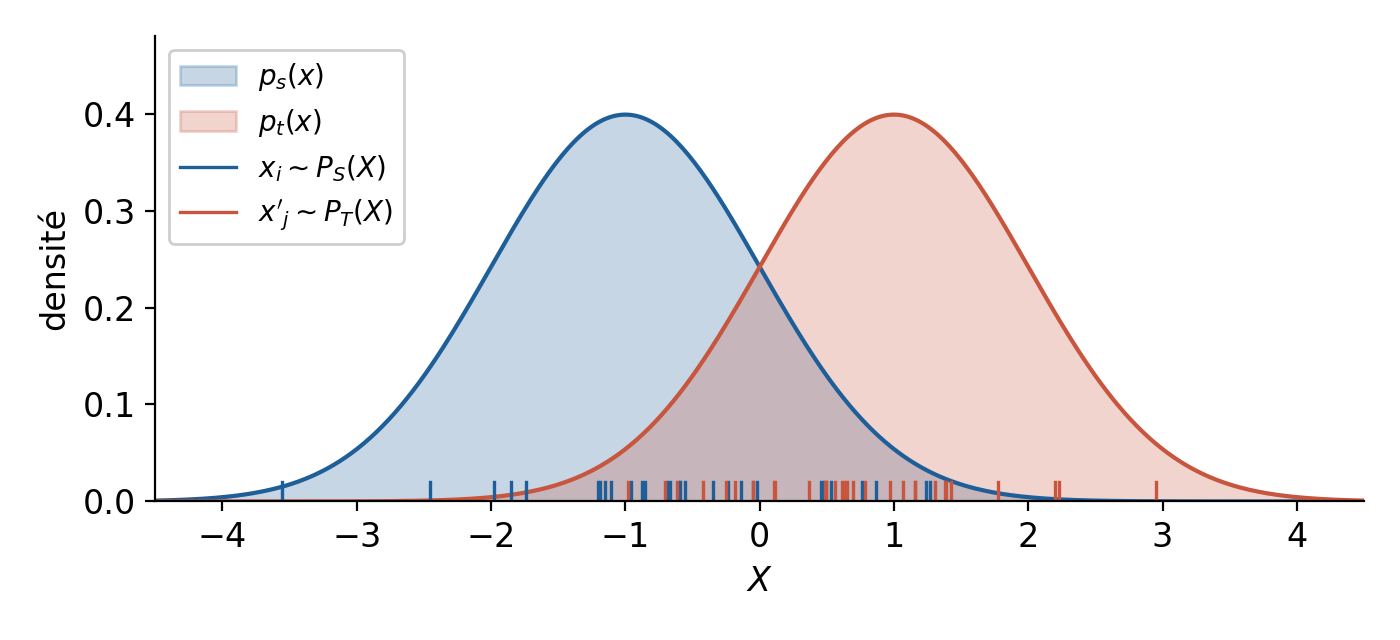
\includegraphics[width=0.72\linewidth]{fig_densities}
\caption{Densités marginales $p_s(x)$ (source) et $p_t(x)$ (cible), avec les échantillons observés
$x_i$ et $x'_j$. Dans cet exemple, $P_S(X)=\mathcal N(-1,1)$ et $P_T(X)=\mathcal N(1,1)$.}
\label{fig:densities}
\end{figure}

Que se passe-t-il si l'on ignore ce décalage et que l'on ajuste un modèle sur la source uniquement ? La
Figure~\ref{fig:regression_bias} en donne la réponse : le modèle capture bien la relation $Y=|X|$
\emph{là où il dispose de données}, c'est-à-dire autour de $x=-1$, mais cette relation, une fois
extrapolée, se révèle biaisée dès qu'on l'évalue sur la zone où vit réellement la population cible,
autour de $x=+1$.

\begin{figure}[h]
\centering
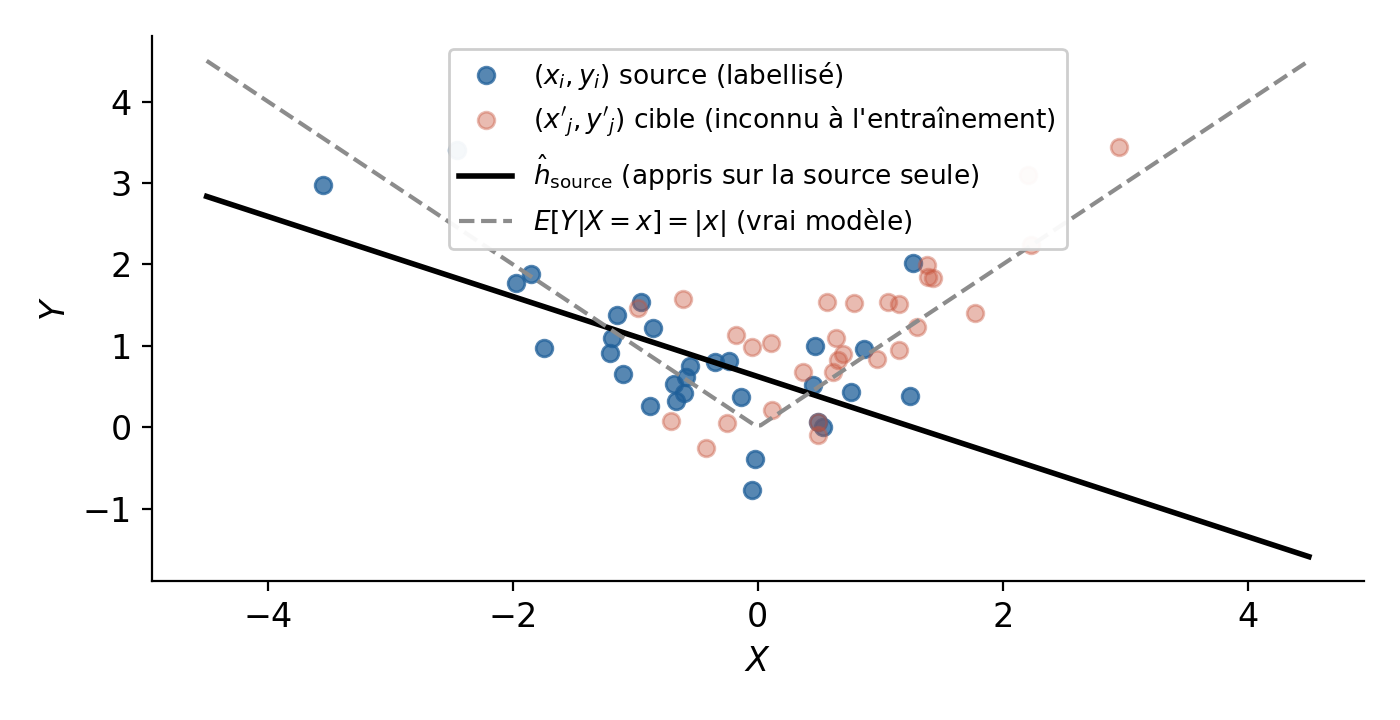
\includegraphics[width=0.85\linewidth]{fig_regression_bias}
\caption{Un modèle appris sur la source seule (noir) est correct près des observations source (bleu)
mais s'écarte du vrai modèle cible $Y=|X|$ (gris pointillé) dans la zone où vit la cible (rouge).}
\label{fig:regression_bias}
\end{figure}

Ce qu'il faut retenir de cet exemple, c'est qu'il ne s'agit en rien d'un problème d'algorithme ou de
capacité du modèle : même un modèle \enquote{parfait} sur la source, au sens du principe ERM, peut se
révéler arbitrairement mauvais sur la cible, dès lors que les deux distributions diffèrent et que la
fonction cible n'est pas correctement extrapolée hors du support source. C'est très exactement le
problème que l'adaptation de domaine cherche à résoudre.

\subsection{Formalisation du problème}

Formalisons à présent ce que nous venons d'observer. Notons $\ell:\Y\times\Y\to\R$ la fonction de perte,
par exemple $\ell(y,y')=\|y-y'\|_2^2$, et $\Hcal$ un espace d'hypothèses --- $\Hcal=\{h:x\mapsto
x\beta^\top,\ \beta\in\R^p\}$ pour des hypothèses linéaires. Le risque cible d'une hypothèse $h\in\Hcal$
s'écrit alors
\[
R_T(h) = \Esp{(x,y)\sim P_T(X,Y)}{\ell(h(x),y)}.
\]
Si l'on disposait d'étiquettes cible $y'_j$, on l'estimerait naturellement par l'estimateur empirique
$\widehat R_T(h) = \frac1n\sum_{j=1}^n \ell(h(x'_j),y'_j)$ --- mais ce n'est précisément pas le cas ici,
puisque nous avons choisi de travailler dans le cadre non supervisé.

\begin{definition}{Problématique de l'UDA}{udaproblem}
L'hypothèse cible optimale est
\[
h^\star = \argmin_{h\in\Hcal} \Esp{(x,y)\sim P_T(X,Y)}{\ell(h(x),y)}.
\]
Le but de l'UDA est de trouver la meilleure estimation possible de $h^\star$ à partir du seul échantillon
source labellisé $S$ et de l'échantillon cible non labellisé $T_X$.
\end{definition}

C'est cette question --- comment approcher $h^\star$ sans jamais voir d'étiquette cible --- qui va
occuper tout le chapitre suivant.

%=====================================================================
\section{Approches instance-based}
\label{sec:instance}
%=====================================================================

Nous allons voir dans ce chapitre que, sous l'hypothèse de covariate shift, le risque cible peut
s'écrire comme un risque source \emph{repondéré} : c'est l'identité fondatrice de toute la famille
d'approches dites \emph{instance-based}. Une fois cette identité établie, la question devient purement
algorithmique --- comment estimer les poids nécessaires ? --- et nous explorerons pour y répondre
plusieurs familles de méthodes, de l'estimation de densité la plus naïve jusqu'au classifieur de domaine,
qui nous servira de pont vers les méthodes profondes du chapitre suivant.

\subsection{Le risque cible est un risque source repondéré}

\begin{proposition}{Changement de mesure}{changemeasure}
Supposons que $P_S(X,Y)$ et $P_T(X,Y)$ admettent des densités $p_s(x,y)$, $p_t(x,y)$, et posons
$w(x,y) = p_t(x,y)/p_s(x,y)$. Alors, pour toute hypothèse $h\in\Hcal$,
\[
\Esp{(x,y)\sim P_T(X,Y)}{\ell(h(x),y)} = \Esp{(x,y)\sim P_S(X,Y)}{w(x,y)\,\ell(h(x),y)}.
\]
\end{proposition}
\begin{proof}
\[
\Esp{P_T}{\ell(h(x),y)} = \int p_t(x,y)\,\ell(h(x),y)\,dx\,dy
 = \int \frac{p_t(x,y)}{p_s(x,y)}\, p_s(x,y)\,\ell(h(x),y)\,dx\,dy
 = \Esp{P_S}{w(x,y)\,\ell(h(x),y)}.\qedhere
\]
\end{proof}

\begin{definition}{Ratio de densités}{densityratio}
Le \textbf{ratio de densités} (ou \emph{importance weight}) est $w(x,y) = p_t(x,y)/p_s(x,y)$, défini pour
$(x,y)$ tel que $p_s(x,y)>0$. On exige que le support de $P_T$ soit inclus dans celui de $P_S$ :
$p_s(x,y)=0 \Rightarrow p_t(x,y)=0$, faute de quoi il existerait une zone cible jamais observée côté
source, qu'aucune repondération ne pourrait corriger.
\end{definition}

Cette identité est élégante, mais elle ne suffit pas encore, en l'état, à construire un algorithme
implémentable : le ratio $w(x,y)$ fait intervenir $p_t(x,y)=p_t(y\mid x)\,p_t(x)$, et donc, \emph{a
priori}, les étiquettes cible --- exactement ce qui nous manque. Il nous faut une hypothèse
supplémentaire pour nous en affranchir.

\subsection{L'hypothèse de covariate shift simplifie tout}

\begin{proposition}{Ratio de densités sous covariate shift}{covshiftratio}
Sous l'hypothèse de covariate shift ($P_T(Y\mid X=x)=P_S(Y\mid X=x)$ pour tout $x$), le ratio de densités
ne dépend plus de $y$ :
\[
w(x,y) = w(x) = \frac{p_t(x)}{p_s(x)}.
\]
\end{proposition}
\begin{proof}
$\displaystyle w(x,y) = \frac{p_t(x,y)}{p_s(x,y)} = \frac{p_t(y\mid x)\,p_t(x)}{p_s(y\mid x)\,p_s(x)}
= \frac{p_t(x)}{p_s(x)}$ car $p_t(y\mid x)=p_s(y\mid x)$ par hypothèse. \qedhere
\end{proof}

C'est un progrès décisif : $w(x)$ ne dépend plus désormais que des \emph{features}, que l'on observe des
deux côtés, source et cible. On peut donc espérer l'estimer sans la moindre étiquette cible --- ce qui
était précisément l'obstacle rencontré à l'instant. Les sondages électoraux en offrent une bonne
illustration : on y suppose que la population sondée vote comme elle répond au sondage, autrement dit que
$P(\text{vote}\mid \text{profil})$ est identique entre l'échantillon interrogé et la population réelle.
Les mesures industrielles en offrent une seconde : la machine de mesure utilisée pour construire le jeu
d'entraînement est supposée avoir le même bruit de mesure que celle utilisée en production. Ce sont là
deux illustrations réelles, dans des contextes très différents, de la même hypothèse de covariate shift.

\begin{proposition}{Risque cible sous covariate shift}{targetriskcov}
Sous covariate shift, en supposant $w(x)$ connu pour tout $x$, le risque cible peut être estimé
uniquement à partir de l'échantillon source labellisé :
\[
R_T(h) = \Esp{(x,y)\sim P_S(X,Y)}{w(x)\,\ell(h(x),y)} \approx \frac1m\sum_{i=1}^m w(x_i)\,\ell(h(x_i),y_i).
\]
\end{proposition}

Récapitulons le chemin parcouru jusqu'ici. Un décalage de domaine implique que risque source et risque
cible sont deux quantités distinctes ; sous covariate shift, le second s'écrit comme le premier
repondéré par $w(x)=p_t(x)/p_s(x)$ ; et comme ce poids ne dépend que des features, il devient estimable
sans la moindre étiquette cible. Reste, précisément, à l'estimer à partir des échantillons $S_X$ et
$T_X$ dont on dispose réellement --- c'est l'objet du reste de ce chapitre.

\subsection{Formulation générale d'une approche instance-based}

\begin{definition}{UDA instance-based}{udainstance}
Une approche instance-based résout le problème d'optimisation en deux temps : on estime
$\widehat w(x_i)$ pour tout $x_i\in S_X$, à partir de $S_X$ et $T_X$ seuls, puis on résout
\[
\widehat h^\star = \argmin_{h\in\Hcal} \frac1m\sum_{i=1}^m \widehat w(x_i)\,\ell(h(x_i),y_i).
\]
\end{definition}

Avant d'étudier comment estimer $\widehat w$ en pratique, traitons l'exercice suivant, qui montre que la
seconde étape --- une fois les poids connus --- se résout de façon entièrement explicite dans le cas
d'une régression linéaire.

\begin{exercise}[Régression pondérée --- solution analytique]
\label{ex:weighted-reg}
Soit $X\in\R^{m\times p}$ la matrice des observations, $Y\in\R^{m}$ le vecteur des cibles, $\ell(y,y')=
(y-y')^2$, $\Hcal=\{h:x\mapsto x\beta^\top,\ \beta\in\R^p\}$, et $w_i = p_t(x_i)/p_s(x_i)$ supposé connu.
Montrez que la solution du problème repondéré
$\beta^\star = \argmin_{\beta} \sum_{i=1}^m w_i (x_i\beta^\top - y_i)^2$
s'écrit, en notant $\Delta=\mathrm{diag}(\sqrt{w_1},\dots,\sqrt{w_m})$,
\[
\beta^\star = \left[X^\top \Delta^2 X\right]^{-1} X^\top \Delta^2 Y.
\]
\end{exercise}
\begin{proof}[Solution]
On écrit $\sum_i w_i (x_i\beta^\top-y_i)^2 = \|\Delta(X\beta^\top - Y)\|_2^2 = \|\Delta X \beta^\top -
\Delta Y\|_2^2$. C'est un problème de moindres carrés ordinaires sur les données transformées $\Delta X$,
$\Delta Y$, dont la solution (en supposant $X^\top\Delta^2 X$ inversible) est
$\beta^\star = [(\Delta X)^\top \Delta X]^{-1}(\Delta X)^\top \Delta Y = [X^\top\Delta^2 X]^{-1}X^\top
\Delta^2 Y$. \qedhere
\end{proof}

La Figure~\ref{fig:reweighting} illustre l'effet de cette repondération sur notre exemple filé : quand
$w(x)$ est connu exactement, le modèle repondéré se rapproche nettement du vrai modèle cible, là où le
modèle source seul en était très éloigné.

\begin{figure}[h]
\centering
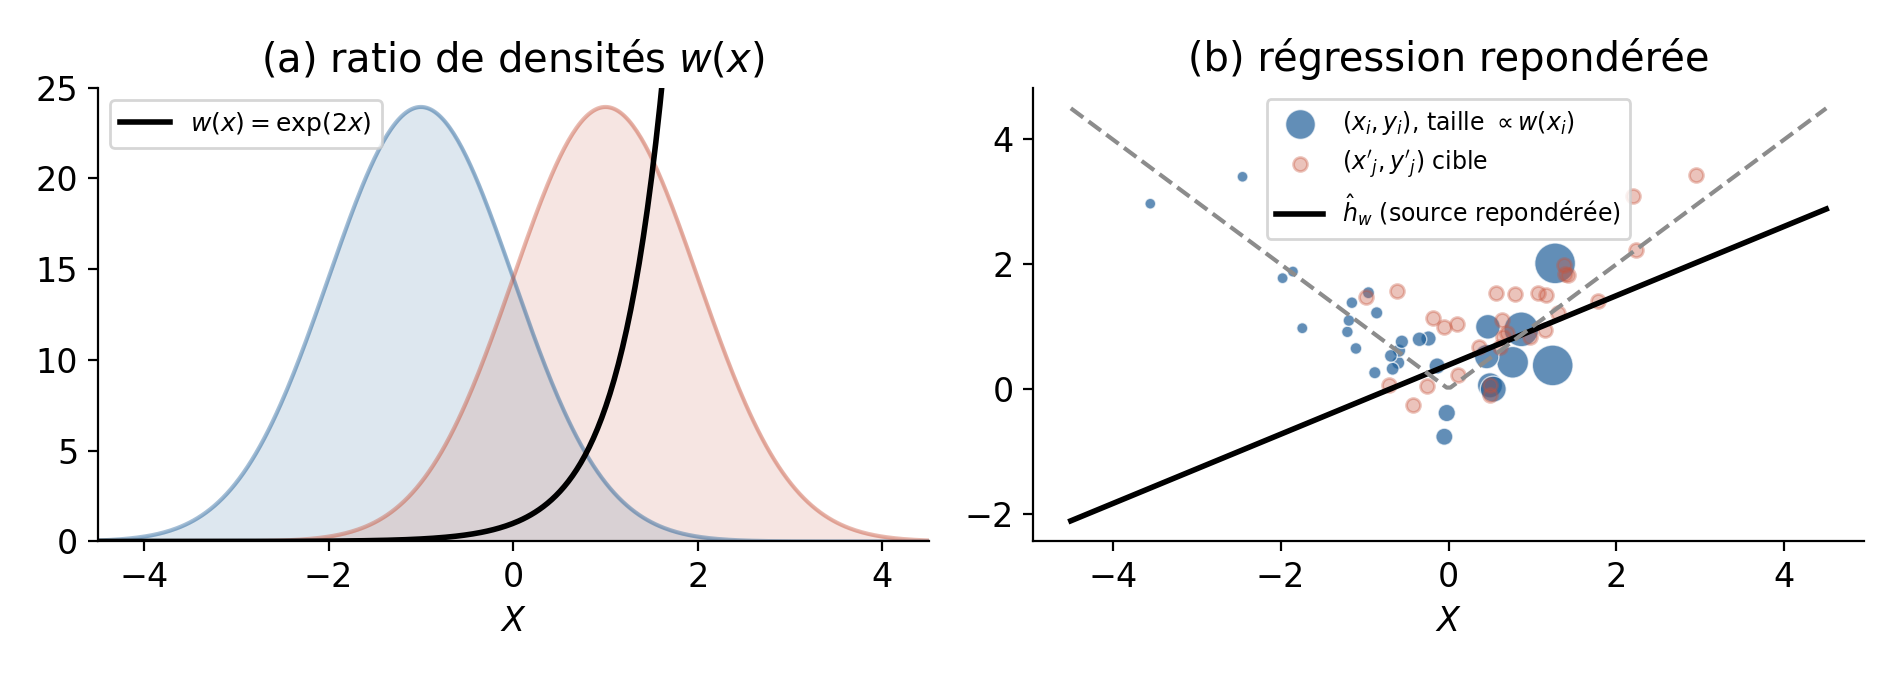
\includegraphics[width=\linewidth]{fig_reweighting}
\caption{(a) Ratio de densités exact $w(x)$ pour deux gaussiennes décalées de moyennes $-1$ et $1$.
(b) Une fois les points source repondérés (taille $\propto w(x_i)$), le modèle appris ($\hat h_w$, noir)
se rapproche du vrai modèle cible (gris pointillé), alors que le modèle non repondéré en était éloigné
(cf. Figure~\ref{fig:regression_bias}).}
\label{fig:reweighting}
\end{figure}

Il faut toutefois garder à l'esprit que, dans cet exemple, $w(x)$ a pu être calculé \emph{analytiquement},
puisque nous connaissions par construction $p_s$ et $p_t$ --- deux gaussiennes aux paramètres fixés à
l'avance. En pratique, ces densités ne sont \textbf{jamais} connues : on n'observe que des échantillons
$S_X$ et $T_X$. La question devient donc : comment estimer $w(x)$ à partir de ces deux échantillons
seuls ? C'est ce que nous allons voir maintenant, en parcourant les quatre grandes familles de méthodes
résumées dans le Tableau~\ref{tab:panorama}.

\subsection{Panorama des méthodes d'estimation de $w(x)$}

\begin{table}[h]
\centering
\small
\begin{tabular}{@{}p{3.6cm}p{4.2cm}p{5.7cm}@{}}
\toprule
\textbf{Famille} & \textbf{Méthodes} & \textbf{Idée} \\
\midrule
Estimation de densité & Paramétrique ; noyaux (KDE) & Estimer $\hat p_s$, $\hat p_t$ séparément, puis
$\hat w = \hat p_t/\hat p_s$ \\
Heuristique & NN weighting \citep{loog2012nearest} & Compter, pour chaque point source, combien de fois
il est plus proche voisin d'un point cible \\
Distribution matching & KLIEP \citep{sugiyama2007direct}, KMM \citep{huang2007correcting} & Chercher
directement $w$ minimisant un écart entre $w\cdot p_s$ et $p_t$ \\
Classifieur de domaine & Linéaire/noyau \citep{bickel2007discriminative}, réseau de neurones
\citep{zhang2018importance} & Relier $w(x)$ à la probabilité que $x$ vienne de la cible plutôt que de la
source \\
\bottomrule
\end{tabular}
\caption{Panorama des approches d'estimation du ratio de densités.}
\label{tab:panorama}
\end{table}

\subsubsection{Estimation de densité paramétrique}

L'idée la plus directe consiste à supposer un modèle de densité $p_s(\theta_s,x)$, $p_t(\theta_t,x)$, par
exemple gaussien, puis à estimer $\theta_s$ et $\theta_t$ par maximum de vraisemblance sur $S_X$ et $T_X$
respectivement, avant de poser $\widehat w(x_i) = p_t(\hat\theta_t,x_i)/p_s(\hat\theta_s,x_i)$. Cette
simplicité a toutefois un coût : elle exige de \emph{deviner} la bonne famille paramétrique. Si la vraie
distribution n'est pas gaussienne --- un mélange de plusieurs modes, une forte asymétrie --- l'estimation
du ratio se retrouve biaisée, parfois radicalement, comme le montre le notebook de TP sur une
distribution exponentielle.

\subsubsection{Estimation de densité par noyaux (KDE)}

Pour s'affranchir du choix d'une famille paramétrique, on peut estimer les densités par noyaux : pour un
noyau $k:\X\times\X\to\R_+$, on pose
\[
\widehat p_s(x) = C_s \sum_{x_i\in S_X} k(x,x_i), \qquad
\widehat p_t(x) = C_t \sum_{x'_j\in T_X} k(x,x'_j),
\]
puis $\widehat w(x_i) = \widehat p_t(x_i)/\widehat p_s(x_i)$. Le noyau gaussien
$k(x,x')=\exp(-\|x-x'\|_2^2/2\sigma^2)$ est le choix le plus courant, le paramètre $\sigma$, appelé
bande passante, étant réglé par validation croisée sur la vraisemblance. Il reste que cette famille de
méthodes --- paramétrique ou à noyaux --- estime les deux densités \emph{séparément} avant d'en prendre
le rapport, ce qui est un problème structurellement plus difficile que d'estimer directement le ratio
lui-même : les erreurs des deux estimations se cumulent, en particulier dans les zones de faible densité
source, où le ratio explose. C'est précisément cette observation qui motive les approches suivantes,
qui cherchent toutes à estimer $w$ \emph{directement}, sans passer par l'étape intermédiaire des deux
densités.

\subsubsection{Heuristique des plus proches voisins}

\begin{definition}{Nearest Neighbors Weighting}{nnweighting}
Pour $K\in\N^*$, notons $V_K(x'_j)$ l'ensemble des $K$ plus proches voisins de $x'_j\in T_X$ dans $S_X$.
Le poids de $x_i\in S_X$ est directement le nombre de fois où il apparaît comme voisin d'un point cible :
\[
\widehat w(x_i) = \mathrm{Card}\big(\{x'_j\in T_X \mid x_i \in V_K(x'_j)\}\big).
\]
\end{definition}

L'intuition qui sous-tend cette heuristique, due à \citet{loog2012nearest}, est la suivante : un point
source \enquote{entouré} de nombreux points cible est sous-représenté relativement à la cible, et doit
donc voir son poids \emph{augmenter}. À l'inverse, un point source isolé de toute observation cible
n'apporte presque rien à la tâche cible, et son poids doit rester proche de zéro. C'est une heuristique
d'une grande simplicité, qui ne fait aucune hypothèse de forme sur les densités sous-jacentes, mais dont
le comportement reste sensible au choix de $K$, comme l'illustre la Figure~\ref{fig:nnweighting}.

\begin{figure}[h]
\centering
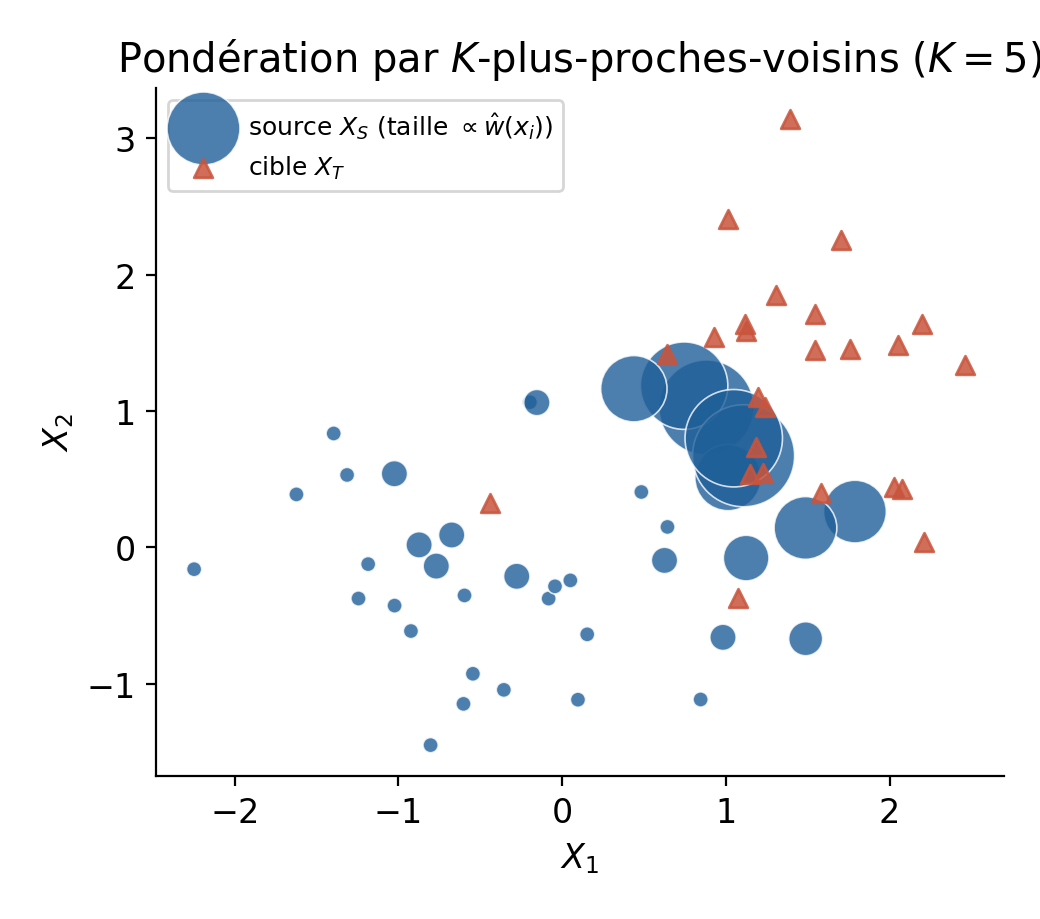
\includegraphics[width=0.55\linewidth]{fig_nnweighting}
\caption{Pondération par plus proches voisins en dimension 2 : les points source (bleu) qui sont souvent
sélectionnés comme voisins de points cible (triangles rouges) reçoivent un poids plus élevé (taille du
marqueur).}
\label{fig:nnweighting}
\end{figure}

\subsubsection{Distribution matching : KLIEP et KMM}

L'idée commune à cette nouvelle famille de méthodes est de renoncer à estimer $p_s$ et $p_t$
séparément, pour chercher \emph{directement} le poids $w$ qui rend la source repondérée $w\cdot p_s$
aussi proche que possible de la cible $p_t$, au sens d'une métrique de proximité $D$ entre distributions :
\[
w^\star = \argmin_{w} D\big(p_t(x),\ w(x)\,p_s(x)\big).
\]
Deux choix de métrique $D$ donnent lieu à deux algorithmes classiques, tous deux encore très employés
aujourd'hui.

\begin{definition}{KLIEP}{kliep}
KLIEP (\emph{Kullback--Leibler Importance Estimation Procedure}, \citealp{sugiyama2007direct}) choisit
$D=\mathrm{KL}$. En écrivant $w$ comme combinaison linéaire de noyaux $w(x)=\sum_{j=1}^b \alpha_j\,
k(x,x'_j)$, le problème devient
\[
\alpha^\star = \argmin_{\alpha\in\R^b} \sum_{x'_i\in T_X} \log\Big(\sum_{j=1}^b \alpha_j\,k(x'_i,x'_j)\Big)
\quad \text{s.c.} \quad \sum_{x_i\in S_X}\sum_{j=1}^b \alpha_j\,k(x_i,x'_j) = 1,\ \alpha\ge 0.
\]
\end{definition}

\begin{definition}{Kernel Mean Matching (KMM)}{kmm}
KMM \citep{huang2007correcting} choisit $D=\mathrm{MMD}$ (\emph{Maximum Mean Discrepancy}), qui compare
deux distributions à travers leurs moments dans un espace de Hilbert à noyau reproduisant. Le problème
d'optimisation devient quadratique :
\[
w^\star = \argmin_{w\in\R^{m},\ w\ge 0,\ w^\top\mathbf 1 = m}\ w^\top K w - 2\kappa^\top w,
\]
où $K_{ij}=k(x_i,x_j)$ pour $x_i,x_j\in S_X$ et $\kappa_i = \frac{m}{n}\sum_{x'_j\in T_X} k(x_i,x'_j)$.
\end{definition}

La MMD compare deux distributions à travers leurs moments : $\Esp{P_S}{X^k}$ contre $\Esp{P_T}{X^k}$
pour tout ordre $k$, l'astuce du noyau permettant de faire ce calcul sans jamais expliciter des moments
d'ordre élevé. Or deux distributions ont tous leurs moments égaux si, et seulement si, elles sont
identiques : c'est très exactement ce principe que KMM exploite pour forcer $w\cdot p_s$ à
\enquote{ressembler} à $p_t$ en tout point, sans jamais avoir à estimer $p_s$ ni $p_t$ séparément. Son
principal avantage pratique est de ne requérir que la résolution d'un programme quadratique convexe, sans
aucune sélection de modèle de densité au préalable.

\subsubsection{Classifieur de domaine (Importance Weighting Classifier)}

Nous arrivons à la dernière famille de méthodes de ce chapitre, et sans doute la plus féconde des
quatre : c'est elle qui inspirera directement les méthodes d'adaptation de domaine profondes du chapitre
suivant.

\begin{definition}{Importance Weighting Classifier}{iwc}
On entraîne un classifieur $\phi:\X\to[0,1]$ à discriminer les échantillons source ($\text{label}=0$) des
échantillons cible ($\text{label}=1$) :
\[
\phi^\star = \argmax_{\phi\in\Phi}\ \Esp{P_S(X)}{\log \phi_0(X)} + \Esp{P_T(X)}{\log \phi_1(X)}
\]
(formulation par entropie croisée), puis on relie le ratio de densités à la sortie de ce classifieur :
\[
w(x) = \frac{1}{\phi(x)} - 1, \qquad \text{où } \phi(x) = \P(\text{domaine}=T\mid X=x).
\]
\end{definition}

L'idée sous-jacente à l'IWC est remarquablement simple, et mérite qu'on la démontre proprement : le ratio
de densités $w(x)$ est directement relié à la probabilité qu'un point $x$ appartienne au domaine cible
plutôt qu'au domaine source, telle qu'estimée par un classifieur entraîné à discriminer les deux.

\begin{exercise}[Justification de l'IWC]
\label{ex:iwc}
Soient $p_s(x)$ et $p_t(x)$ telles que $\mathrm{supp}(p_t)\subset\mathrm{supp}(p_s)$, et soit $\phi^\star$
le classifieur de domaine optimal pour la perte d'entropie croisée :
\[
\phi^\star = \argmax_{\phi}\ \Esp{P_S(X)}{\log\phi(X)} + \Esp{P_T(X)}{\log(1-\phi(X))}.
\]
Montrez que $w(x) = p_t(x)/p_s(x) = 1/\phi^\star(x) - 1$.
\end{exercise}
\begin{proof}[Solution]
En développant les espérances en intégrales,
\[
\phi^\star = \argmax_\phi \int_\X \big(p_s(x)\log\phi(x) + p_t(x)\log(1-\phi(x))\big)\,dx.
\]
Pour chaque $x$ fixé, on maximise point par point $g(\phi) = p_s(x)\log\phi + p_t(x)\log(1-\phi)$ en
$\phi\in(0,1)$ : $g'(\phi) = p_s(x)/\phi - p_t(x)/(1-\phi) = 0 \iff \phi^\star(x) = \dfrac{p_s(x)}{p_s(x)+
p_t(x)}$. On vérifie $g''<0$ (maximum). On en déduit
\[
\frac{1}{\phi^\star(x)} - 1 = \frac{p_s(x)+p_t(x)}{p_s(x)} - 1 = \frac{p_t(x)}{p_s(x)} = w(x). \qedhere
\]
\end{proof}

Une mise en garde s'impose ici, car elle donne lieu à un piège classique en TP : dans cet exercice,
$\phi(x)$ est défini comme $\P(\text{domaine}=S\mid x)$ et non comme $\P(\text{domaine}=T\mid x)$, afin de
retrouver exactement la formule du cours de référence sur lequel s'appuie cet exercice. Selon la
convention choisie pour l'étiquetage $0/1$ des domaines source et cible, le poids s'écrit donc soit
$w(x)=1/\phi(x)-1$, soit $w(x)=\phi(x)/(1-\phi(x))$ : il faut \textbf{toujours} vérifier la convention en
vigueur avant d'implémenter quoi que ce soit, sous peine d'inverser purement et simplement le sens de la
repondération.

\begin{figure}[h]
\centering
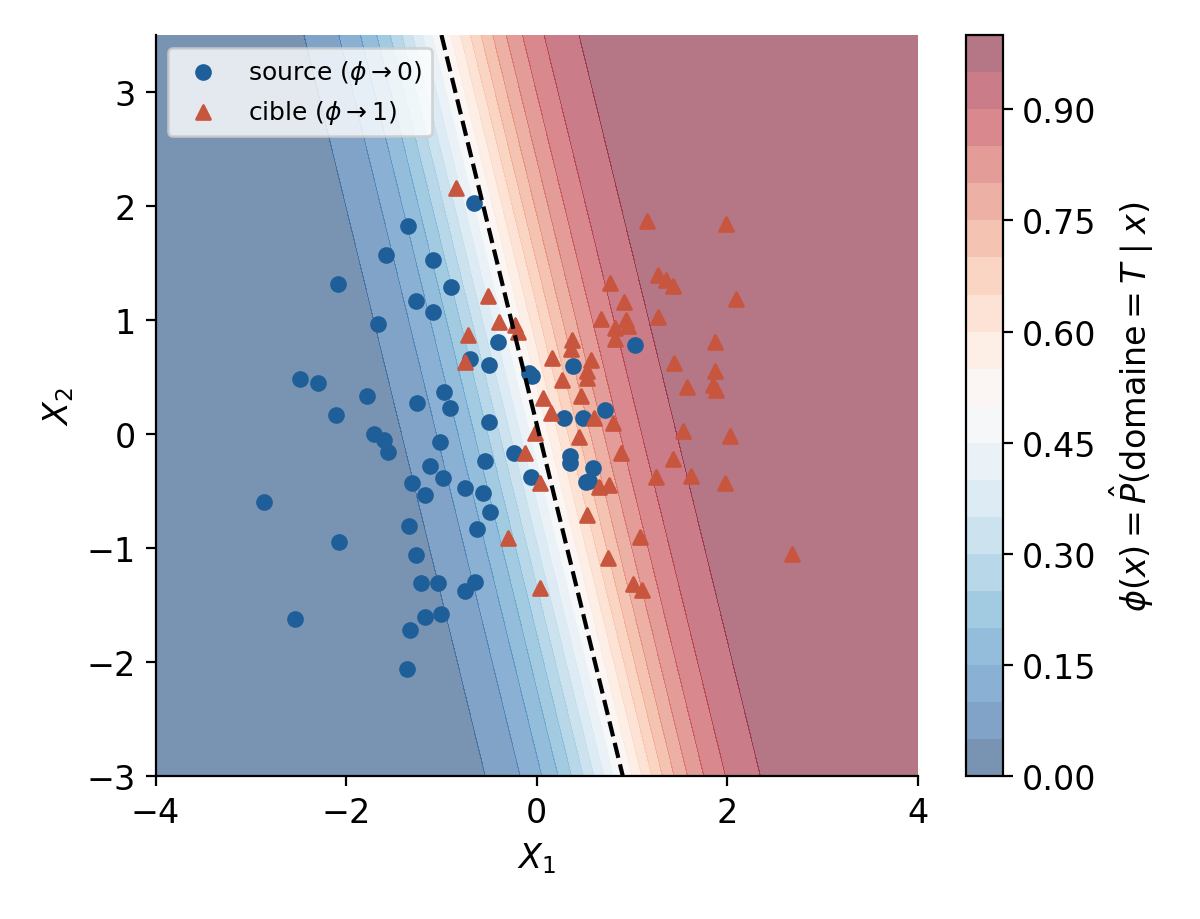
\includegraphics[width=0.62\linewidth]{fig_domainclassifier}
\caption{Un classifieur de domaine $\phi(x)=\hat\P(T\mid x)$ (ici une régression logistique) sépare les
points source (bleu, $\phi\to 0$) des points cible (rouge, $\phi\to 1$). Le ratio de densités
$w(x)=\phi(x)/(1-\phi(x))$ (convention $0=S,1=T$) explose quand $\phi(x)\to 1$, c'est-à-dire dans les
zones \enquote{typiquement cible}.}
\label{fig:domainclassifier}
\end{figure}

Le choix de la classe de classifieurs $\Phi$ pilote directement la complexité de la repondération
obtenue : un classifieur linéaire produira un $w$ \enquote{simple}, correspondant à une frontière
linéaire entre les deux nuages de points, tandis qu'un réseau de neurones produira un $w$ beaucoup plus
flexible --- au risque, si le classifieur devient trop expressif par rapport à la taille des échantillons
dont on dispose, de surapprendre et de produire des poids extrêmes concentrés sur quelques points isolés
seulement.

\subsection{Et quand le covariate shift ne tient pas, ou que les supports ne se recouvrent pas ?}

Il convient de conclure ce chapitre par deux limites structurelles, communes à l'ensemble des méthodes
que nous venons de voir. La première est logique : si $P_S(Y\mid X)\neq P_T(Y\mid X)$, c'est-à-dire si
l'hypothèse de covariate shift ne tient plus, repondérer les instances ne corrige absolument rien, car
on ne fait alors que repondérer la distribution des $X$, sans toucher à la relation $X\to Y$ elle-même,
qui a pourtant changé. La seconde est numérique : si $p_s(x)\approx 0$ dans une région où $p_t(x)>0$, le
ratio $w(x)=p_t(x)/p_s(x)$ explose, quelques points source reçoivent alors un poids disproportionné, et
l'estimateur repondéré devient très instable, au sens d'une variance élevée. C'est de loin le symptôme le
plus fréquent d'échec pratique des méthodes instance-based, et nous y reviendrons de façon quantitative
au TD, à travers la notion d'\emph{Effective Sample Size}.

C'est précisément pour répondre à ces deux limites que la littérature s'est progressivement tournée vers
les approches \emph{feature-based} : plutôt que de repondérer les points existants, on cherche un espace
de représentation commun dans lequel les deux domaines se recouvrent davantage. C'est l'un des fils
conducteurs du chapitre suivant.

%=====================================================================
\section{Travaux récents : théorie et pratique}
\label{sec:recent}
%=====================================================================

Ce dernier chapitre répond à deux questions restées jusqu'ici en suspens. La première est théorique :
\emph{pourquoi} les méthodes instance-based --- et leurs cousines feature-based --- fonctionnent-elles
réellement, et sous quelles conditions précises peut-on garantir qu'elles amélioreront le risque cible ?
Nous y répondrons à l'aide des bornes de généralisation qui relient formellement risque source et risque
cible. La seconde question est pratique : quelles sont, aujourd'hui, les grandes familles d'algorithmes
qui dominent l'adaptation de domaine en dehors du cadre instance-based que nous avons étudié en détail ?
Nous parcourrons pour cela un panorama volontairement large, des réseaux adversariaux au transport
optimal, en passant par l'adaptation au moment même du test.

\subsection{Pourquoi une borne de généralisation ?}

Jusqu'ici, nous disposons d'une méthode --- repondérer --- mais d'aucune garantie théorique : rien ne
nous dit, pour une paire de domaines donnée, à quel point on peut espérer que $R_T(h)$ se rapproche de
$\widehat R_S(h)$, repondéré ou non. Les bornes de généralisation en adaptation de domaine répondent
précisément à cette question, en général sous une forme structurée en trois termes :
\[
R_T(h) \ \le\ R_S(h) \ + \ (\text{terme de divergence entre domaines}) \ + \ (\text{terme irréductible}).
\]
Les deux sections suivantes détaillent deux instances célèbres de cette forme générale : la borne de
Ben-David et al., historiquement la première, puis son pendant PAC-Bayésien, souvent plus fin en
pratique.

\subsection{La borne $\Hcal\Delta\Hcal$ de Ben-David et al.}

\begin{definition}{$\Hcal$-divergence}{hdiv}
Pour une classe d'hypothèses $\Hcal$ vue comme classe de classifieurs binaires $\X\to\{0,1\}$, la
\textbf{$\Hcal$-divergence} entre deux distributions marginales $D_S=P_S(X)$ et $D_T=P_T(X)$ est
\[
d_{\Hcal}(D_S,D_T) = 2\sup_{h\in\Hcal}\ \Big|\P_{x\sim D_S}\big[h(x)=1\big] - \P_{x\sim D_T}\big[h(x)=1\big]\Big|.
\]
\end{definition}

Cette quantité mesure à quel point le \emph{meilleur} classifieur de la famille $\Hcal$ parvient à
distinguer un point source d'un point cible. Si $D_S=D_T$, aucun classifieur ne peut faire mieux que le
hasard, et $d_\Hcal=0$ ; plus les domaines sont \enquote{séparables}, plus $d_\Hcal$ se rapproche de son
maximum, égal à $2$. On retrouve ici, sous un jour nouveau, exactement l'idée du classifieur de domaine
introduit au chapitre précédent : entraîner un classifieur source-vs-cible n'était donc pas qu'une astuce
pour estimer $w(x)$, c'est littéralement une façon d'estimer empiriquement $d_\Hcal$.

Pour formuler une borne exploitable sur une classe d'hypothèses $\Hcal$ donnée --- et pas seulement sur
des classifieurs binaires --- il faut introduire une variante légèrement plus subtile de cette
divergence.

\begin{definition}{Divergence $\Hcal\Delta\Hcal$}{hdeltah}
On introduit la classe symétrisée $\Hcal\Delta\Hcal = \{h\oplus h' : h,h'\in\Hcal\}$, c'est-à-dire le
\texttt{XOR} de deux hypothèses de $\Hcal$ --- l'ensemble des régions de désaccord entre deux hypothèses
de $\Hcal$ ---, et
\[
\dHDelta(D_S,D_T) = 2\sup_{h,h'\in\Hcal}\ \Big|\P_{D_S}\big[h(x)\neq h'(x)\big] - \P_{D_T}\big[h(x)\neq
h'(x)\big]\Big|.
\]
\end{definition}

Nous disposons à présent de tous les ingrédients pour énoncer le résultat central de \citet{ben2010theory}.

\begin{theorem}{Borne de Ben-David et al. (2010)}{bendavid}
Soit $\Hcal$ une classe d'hypothèses de classification, $R_S(h)$, $R_T(h)$ les risques (en $0/1$-loss)
sous les distributions jointes source et cible. Notons
\[
\lambda_\Hcal = \min_{h\in\Hcal}\big(R_S(h)+R_T(h)\big)
\]
le risque joint optimal atteignable (irréductible : c'est le meilleur compromis possible entre les deux
domaines). Alors, pour tout $h\in\Hcal$,
\[
R_T(h) \ \le\ R_S(h) \ + \ \tfrac12\, \dHDelta(D_S,D_T) \ + \ \lambda_\Hcal.
\]
\end{theorem}

\begin{proofsketch}
On ne reprend pas ici la démonstration complète, disponible dans \citet{ben2010theory}, mais seulement
son idée directrice. On introduit l'hypothèse jointe optimale $h^\star = \argmin_{h}(R_S(h)+R_T(h))$, et
on décompose $R_T(h) \le R_T(h^\star) + \P_{D_T}[h\neq h^\star]$ par l'inégalité triangulaire pour le
désaccord entre classifieurs. On répète le même argument côté source, puis on relie $\P_{D_T}[h\neq
h^\star]$ et $\P_{D_S}[h\neq h^\star]$ via la définition de $\dHDelta$, vue comme borne \emph{sup} sur les
désaccords, ce qui fait apparaître le terme de divergence recherché.
\end{proofsketch}

Cette borne dit quelque chose de très concret : minimiser le risque cible revient à minimiser
simultanément, d'une part, le risque source, et d'autre part la divergence entre les deux domaines,
mesurée dans l'espace de représentation utilisé. Le terme $\lambda_\Hcal$ rappelle, quant à lui,
qu'aucune méthode ne peut faire mieux que le meilleur compromis atteignable par la classe $\Hcal$ : si
les tâches sont fondamentalement incompatibles, dans un cas extrême de concept shift par exemple, aucune
astuce algorithmique ne saurait sauver la situation.

Il faut enfin noter que la $\Hcal\Delta\Hcal$-divergence ne peut, en toute rigueur, pas être calculée
exactement, puisqu'elle porte sur un supremum sur une classe de fonctions en général infinie. Elle admet
toutefois un proxy empirique parfaitement calculable : on entraîne un classifieur $\phi$ à discriminer
$S_X$ de $T_X$ --- exactement le classifieur de domaine du chapitre précédent --- et l'on estime
\[
\hat d_\Hcal(S_X,T_X) = 2\Big(1 - 2\min_{\phi\in\Hcal}\big[\mathrm{err}(\phi)\big]\Big),
\]
où $\mathrm{err}(\phi)\in[0,\tfrac12]$ désigne le taux d'erreur du \emph{meilleur} classifieur de domaine
de $\Hcal$ à séparer source et cible : un classifieur incapable de faire mieux que le hasard a
$\mathrm{err}(\phi)=1/2$, ce qui redonne bien $\hat d_\Hcal=0$, tandis qu'un classifieur parfait a
$\mathrm{err}(\phi)=0$, ce qui redonne $\hat d_\Hcal=2$, la valeur maximale. C'est la \textbf{proxy
$\mathcal A$-distance} de \citet{ben2010theory}. Un classifieur de domaine qui se trompe beaucoup, proche
du hasard, signale ainsi des domaines proches, tandis qu'un classifieur qui sépare parfaitement signale
des domaines très éloignés --- exactement l'intuition que suggérait déjà la Figure~\ref{fig:domainclassifier}.

\subsection{Bornes PAC-Bayésiennes pour l'adaptation de domaine}

Les bornes de type Ben-David portent sur un unique classifieur $h$. L'approche PAC-Bayésienne, elle,
raisonne sur une \emph{distribution} $Q$ de classifieurs --- un vote de majorité --- et permet d'obtenir
des bornes souvent plus fines en pratique.

\begin{definition}{Cadre PAC-Bayésien pour le DA \citep{germain2013pacbayesian}}{pbda}
Soit $\Hcal$ une classe d'hypothèses, $Q$ une distribution (\emph{posterior}) sur $\Hcal$, et $P$ un
\emph{prior} indépendant des données. On définit le risque de Gibbs sous $Q$,
$R_\D(Q) = \Esp{h\sim Q}{R_\D(h)}$ pour $\D\in\{S,T\}$, et le \textbf{désaccord de domaine} sous $Q$ :
\[
\mathrm{dis}_T(Q) = \Esp{(h,h')\sim Q^2}{\P_{x\sim D_T}\big[h(x)\neq h'(x)\big]}.
\]
\end{definition}

\begin{theorem}{Borne PAC-Bayésienne pour l'adaptation de domaine \citep{germain2013pacbayesian,germain2016new}}{pbdabound}
Sous des hypothèses techniques usuelles (perte bornée, échantillons i.i.d.), avec probabilité au moins
$1-\delta$ sur le tirage de $S$ et $T_X$, pour tout posterior $Q$ sur $\Hcal$ :
\[
R_T(Q) \ \le\ R_S(Q) \ + \ \tfrac12\, \mathrm{dis}_T(Q) \ + \ \lambda(Q)
\ + \ O\!\left(\sqrt{\frac{\KL(Q\|P) + \log\frac1\delta}{m}}\right),
\]
où $\lambda(Q)$ est, comme précédemment, un terme irréductible dépendant du meilleur compromis
source/cible atteignable sous $Q$, et $\KL(Q\|P)$ est la divergence de Kullback-Leibler entre le
posterior appris et le prior.
\end{theorem}

La structure de cette borne est exactement la même que celle de Ben-David --- risque source, plus
divergence de domaine, plus terme irréductible --- mais deux différences comptent en pratique. D'une
part, le désaccord $\mathrm{dis}_T(Q)$ peut non seulement être estimé sans étiquette cible, mais aussi
être optimisé directement en apprenant $Q$, plutôt que de se contenter d'un simple proxy de classifieur
de domaine. D'autre part, le terme de complexité $\KL(Q\|P)$ contrôle explicitement le compromis
biais/variance : un posterior $Q$ trop éloigné du prior $P$, donc très \enquote{spécialisé}, dégrade la
garantie théorique même s'il minimise parfaitement les deux premiers termes. C'est ce même principe qui
sous-tend les certificats PAC-Bayésiens pour les méthodes d'ensemble étudiées ailleurs dans ce master.
Ces bornes ont depuis été raffinées par \citet{germain2016new}, qui en propose des versions à la fois
plus serrées et calculables pour des posteriors linéaires, utiles par exemple pour des SVM ou des modèles
linéaires adaptés au domaine ; plus récemment encore, dans les années 2020, une ligne de travaux combine
ce cadre avec le transport optimal --- que nous verrons plus bas --- pour obtenir des bornes exploitant
directement une distance de Wasserstein entre domaines, souvent plus facile à estimer en haute dimension
qu'une divergence de nature combinatoire.

\subsection{Une mise en garde théorique récente : les limites du \enquote{domain-invariant}}

\begin{recent}
Une intuition très répandue depuis Ben-David et al. veut que, si l'on apprend une représentation où
$\hat d_\Hcal(S,T)\approx 0$ --- des domaines devenus indistinguables --- alors un bon transfert soit
garanti. \citet{zhao2019learning} montrent que cette intuition est \textbf{fausse en général sous target
shift} : rendre les représentations totalement invariantes au domaine peut en réalité \emph{augmenter}
l'erreur jointe minimale $\lambda_\Hcal$ elle-même, en détruisant l'information nécessaire pour
distinguer les classes entre elles. Les auteurs établissent même des bornes \emph{inférieures},
c'est-à-dire des résultats d'impossibilité, dès lors que les proportions de classes diffèrent trop entre
source et cible. C'est un rappel salutaire : la borne de Ben-David constitue une condition
\emph{suffisante} pour contrôler un terme du risque, non une recette universelle --- et ce résultat
explique en partie pourquoi le simple fait de \enquote{tromper un classifieur de domaine}, comme le fait
DANN que nous introduisons ci-dessous, échoue parfois en présence d'un target shift marqué.
\end{recent}

\subsection{DANN : rendre les représentations invariantes par apprentissage adversarial}

\begin{recent}
\citet{ganin2015dann} proposent une opérationnalisation directe de la borne de Ben-David : au lieu de
repondérer des instances dans l'espace des features d'origine, on apprend un \textbf{extracteur de
features} $G_f$, un réseau de neurones, tel qu'un classifieur de labels $G_y$ appliqué sur $G_f(x)$
minimise le risque source comme d'habitude, tandis qu'un classifieur de domaine $G_d$ appliqué sur
$G_f(x)$ ne parvient plus, lui, à distinguer source et cible --- ce qui, par construction, revient
exactement à minimiser le proxy empirique de $\dHDelta$ introduit plus haut. L'astuce d'implémentation
qui rend cela possible, le \textbf{Gradient Reversal Layer}, permet d'entraîner les trois morceaux du
réseau ($G_f$, $G_y$, $G_d$) en une seule et même descente de gradient : le gradient de la perte de
$G_d$ est simplement \emph{inversé} au moment où il traverse $G_f$ lors de la rétropropagation, ce qui
revient à faire, du point de vue de $G_f$, un pas de \emph{maximisation} de l'erreur du classifieur de
domaine, tout en continuant, du point de vue de $G_d$ lui-même, une descente de gradient tout à fait
classique. On obtient ainsi un jeu à deux joueurs, de type minimax, sans jamais avoir à implémenter de
double boucle d'optimisation.
\end{recent}

DANN peut ainsi se lire comme l'IWC du chapitre précédent, mais employé pour apprendre une représentation
plutôt que pour repondérer des instances déjà existantes : le même classifieur de domaine $\phi$, la même
intuition selon laquelle un bon transfert rend source et cible indiscernables, mais une optimisation qui
porte désormais sur les \emph{features} elles-mêmes plutôt que sur de simples poids scalaires. Cette
extension permet de traiter des situations où aucune repondération d'instances ne suffirait --- par
exemple lorsque les supports sont initialement disjoints --- au prix, toutefois, de la mise en garde
énoncée à l'instant.

\subsection{Panorama pratique complémentaire}

Au-delà de DANN, plusieurs autres directions structurent aujourd'hui la pratique de l'adaptation de
domaine, chacune répondant à une limite différente des méthodes vues dans ce cours.

\begin{recent}
\textbf{Alignement de moments (Deep CORAL, MMD-based deep DA).} Plutôt qu'un jeu adversarial, on peut
ajouter directement à la perte d'entraînement un terme qui pénalise l'écart entre les statistiques des
features source et cible --- la covariance pour CORAL \citep{sun2016coral}, la MMD pour DAN
\citep{long2015dan} --- ce qui constitue une extension directe de KMM à l'espace des features appris
plutôt qu'à l'espace d'entrée brut.

\textbf{Transport optimal pour l'adaptation de domaine.} \citet{courty2017optimal} formulent
l'adaptation de domaine comme un problème de \emph{transport optimal} : on cherche le plan de transport
$\gamma$ le moins coûteux qui déplace la masse de $p_s$ vers $p_t$, avant d'apprendre conjointement le
classifieur et ce plan de transport (\emph{JDOT}). La distance de Wasserstein qui en résulte a
l'avantage d'une interprétation géométrique directe --- elle mesure un \enquote{coût de déplacement}
plutôt qu'un simple rapport de densités --- et se comporte souvent mieux en haute dimension que KL ou
MMD lorsque les supports se recouvrent peu, exactement la limite pointée en fin de
Section~\ref{sec:instance}.

\textbf{Auto-apprentissage et pseudo-labellisation.} Une fois un premier modèle adapté disponible, rien
n'empêche de lui faire prédire des \emph{pseudo-étiquettes} sur la cible, de ne garder que les
prédictions les plus confiantes, puis de réentraîner en semi-supervisé sur la source et la cible ainsi
pseudo-labellisée. C'est un principe d'une grande simplicité, itéré et raffiné (seuils adaptatifs par
classe, par exemple), redevenu très compétitif sur les benchmarks de vision récents.

\textbf{Test-Time Adaptation (TENT).} \citet{wang2021tent} posent un cadre encore plus contraint : au
moment du test, on ne dispose \textbf{ni des données source, ni d'aucune étiquette}, seulement d'un flux
de données cible non labellisées et d'un modèle déjà entraîné. TENT adapte alors uniquement les
paramètres des couches de normalisation (\emph{batch normalization}) du réseau, en minimisant l'entropie
des prédictions sur les lots cible observés au fil du temps --- une adaptation \enquote{à la volée}, sans
jamais revoir la source.

\textbf{Adaptation de domaine avec des modèles de fondation.} Depuis 2022, les modèles pré-entraînés à
grande échelle, CLIP et ses variantes en tête, changent sensiblement la donne : leur espace de
représentation, appris sur des milliards de paires image-texte, se révèle déjà remarquablement robuste
aux décalages de domaine visuels usuels. Les travaux les plus récents, entre 2023 et 2025, portent ainsi
moins sur l'alignement explicite de distributions que sur le \emph{prompt tuning} ou l'ajout de petits
adaptateurs légers, pour spécialiser ce modèle générique à la tâche cible avec très peu, voire aucune,
donnée cible étiquetée --- une forme de transfert où le \enquote{domaine source} est devenu si large et
si divers que le décalage résiduel vers presque n'importe quelle cible réaliste devient gérable par un
ajustement minimal.
\end{recent}

Retenons de ce chapitre l'essentiel. La borne de Ben-David formalise le compromis entre risque source,
divergence entre domaines, et risque joint irréductible, un socle théorique commun à presque toute la
littérature de l'adaptation de domaine. Le classifieur de domaine n'y est d'ailleurs pas qu'un outil
pratique : c'est un véritable estimateur de la $\Hcal\Delta\Hcal$-divergence, ce qui explique directement
pourquoi une méthode comme DANN fonctionne. Les bornes PAC-Bayésiennes généralisent ce cadre à des votes
de majorité, avec un contrôle explicite de la complexité via $\KL(Q\|P)$ ; mais rendre les représentations
\enquote{invariantes au domaine} n'est en rien une garantie universelle, puisque sous target shift
marqué, cela peut au contraire se révéler contre-productif, comme l'ont montré Zhao et al. en 2019. Le
transport optimal, la pseudo-labellisation, le test-time adaptation et les modèles de fondation
constituent enfin quatre directions actuelles particulièrement actives, chacune apportant sa propre
réponse à une limite spécifique des méthodes étudiées dans ce cours.

%=====================================================================
\section{Conclusion}
%=====================================================================

L'adaptation de domaine part d'un constat simple --- un modèle entraîné sur une distribution $P_S$ n'a
aucune garantie de bien fonctionner sous une autre distribution $P_T$ --- et propose une famille
d'outils pour restaurer cette garantie, sous des hypothèses explicites sur la relation entre $P_S$ et
$P_T$. Les approches instance-based, sous l'hypothèse de covariate shift, offrent la voie la plus directe
et la plus interprétable : repondérer les exemples source pour que leur distribution repondérée
\enquote{ressemble} à la cible. Le principal défi pratique reste l'estimation de ce poids, de la simple
estimation de densité au classifieur de domaine, en passant par le distribution matching. Les bornes de
Ben-David et les bornes PAC-Bayésiennes expliquent pourquoi ces méthodes marchent, et surtout quand elles
risquent d'échouer, et se retrouvent, décennie après décennie, au cœur des méthodes profondes les plus
récentes --- DANN, transport optimal, test-time adaptation. Retenez surtout ceci : avant d'appliquer
n'importe quelle méthode d'adaptation de domaine, demandez-vous quelle hypothèse de correspondance
source/cible, parmi celles de la Section~\ref{sec:assumptions}, est plausible pour votre problème --- car
c'est elle qui déterminera, en dernier ressort, si la méthode a une chance de fonctionner.

\appendix
\section{Réponses aux questions d'auto-évaluation}
\label{app:answers}
\begin{enumerate}
\item[Q1.1] Le domaine change (l'apparence des images, donc $P(X)$) ; si la tâche reste
\enquote{reconnaître les mêmes objets}, $P(Y\mid X)$ ne change pas en principe --- c'est un cas typique
de covariate shift.
\item[Q1.2] Une campagne de recrutement médical qui change de tranche d'âge cible : $P(X\mid Y)$ (profil
des patients avec/sans la pathologie) reste stable, mais la proportion de patients malades change selon
la population recrutée.
\item[Q1.3] Plus les domaines sont différents, plus le meilleur compromis atteignable $\lambda_\Hcal$
(risque joint minimal) risque d'être élevé lui-même : même la meilleure méthode ne peut pas faire mieux
que cette limite structurelle.
\end{enumerate}

\bibliographystyle{plainnat}
\begin{thebibliography}{99}

\bibitem[Ben-David et al.(2010)]{ben2010theory}
Ben-David, S., Blitzer, J., Crammer, K., Kulesza, A., Pereira, F., and Vaughan, J. W. (2010).
A theory of learning from different domains.
\textit{Machine Learning}, 79(1-2):151--175.

\bibitem[Bickel et al.(2007)]{bickel2007discriminative}
Bickel, S., Brückner, M., and Scheffer, T. (2007).
Discriminative learning for differing training and test distributions.
In \textit{Proceedings of the 24th ICML}, pages 81--88.

\bibitem[Courty et al.(2017)]{courty2017optimal}
Courty, N., Flamary, R., Habrard, A., and Rakotomamonjy, A. (2017).
Joint distribution optimal transportation for domain adaptation.
In \textit{Advances in Neural Information Processing Systems (NeurIPS)}, 30.

\bibitem[Ganin and Lempitsky(2015)]{ganin2015dann}
Ganin, Y. and Lempitsky, V. (2015).
Unsupervised domain adaptation by backpropagation.
In \textit{Proceedings of the 32nd ICML}, pages 1180--1189.

\bibitem[Germain et al.(2013)]{germain2013pacbayesian}
Germain, P., Habrard, A., Laviolette, F., and Morvant, E. (2013).
A PAC-Bayesian approach for domain adaptation with specialization to linear classifiers.
In \textit{Proceedings of the 30th ICML}, pages 738--746.

\bibitem[Germain et al.(2016)]{germain2016new}
Germain, P., Habrard, A., Laviolette, F., and Morvant, E. (2016).
A new PAC-Bayesian perspective on domain adaptation.
In \textit{Proceedings of the 33rd ICML}, pages 859--868.

\bibitem[Huang et al.(2007)]{huang2007correcting}
Huang, J., Gretton, A., Borgwardt, K., Schölkopf, B., and Smola, A. J. (2007).
Correcting sample selection bias by unlabeled data.
In \textit{Advances in Neural Information Processing Systems (NeurIPS)}, 19, pages 601--608.

\bibitem[Long et al.(2015)]{long2015dan}
Long, M., Cao, Y., Wang, J., and Jordan, M. (2015).
Learning transferable features with deep adaptation networks.
In \textit{Proceedings of the 32nd ICML}, pages 97--105.

\bibitem[Loog(2012)]{loog2012nearest}
Loog, M. (2012).
Nearest neighbor-based importance weighting.
In \textit{IEEE International Workshop on Machine Learning for Signal Processing}, pages 1--6.

\bibitem[Sugiyama et al.(2007)]{sugiyama2007direct}
Sugiyama, M., Nakajima, S., Kashima, H., Bünau, P. v., and Kawanabe, M. (2007).
Direct importance estimation with model selection and its application to covariate shift adaptation.
In \textit{Advances in Neural Information Processing Systems (NeurIPS)}, 20, pages 1433--1440.

\bibitem[Sun and Saenko(2016)]{sun2016coral}
Sun, B. and Saenko, K. (2016).
Deep CORAL: correlation alignment for deep domain adaptation.
In \textit{ECCV Workshops}, pages 443--450.

\bibitem[Wang et al.(2021)]{wang2021tent}
Wang, D., Shelhamer, E., Liu, S., Olshausen, B., and Darrell, T. (2021).
Tent: fully test-time adaptation by entropy minimization.
In \textit{International Conference on Learning Representations (ICLR)}.

\bibitem[Zhang et al.(2018)]{zhang2018importance}
Zhang, J., Ding, Z., Li, W., and Ogunbona, P. (2018).
Importance weighted adversarial nets for partial domain adaptation.
In \textit{Proceedings of the IEEE Conference on Computer Vision and Pattern Recognition (CVPR)}, pages
8156--8164.

\bibitem[Zhao et al.(2019)]{zhao2019learning}
Zhao, H., des Combes, R. T., Zhang, K., and Gordon, G. (2019).
On learning invariant representations for domain adaptation.
In \textit{Proceedings of the 36th ICML}, pages 7523--7532.

\bibitem[Zhuang et al.(2021)]{zhuang2021comprehensive}
Zhuang, F., Qi, Z., Duan, K., Xi, D., Zhu, Y., Zhu, H., Xiong, H., and He, Q. (2021).
A comprehensive survey on transfer learning.
\textit{Proceedings of the IEEE}, 109(1):43--76.

\end{thebibliography}

\end{document}
